%=================
\chapter{Sprint 2}
%=================


%------------------------
\section{Sprint Planning}
%------------------------
The first sprint resulted in a solid core for the utility. During the next sprint iteration, the core will be extended with more advanced functionality. After this sprint, the utility will have most of the functionalities it need to work in a real environment, and will probably be able to aid Thales in some of their operations.

Not yet understanding the complexity of all the requirements in the sprint backlog, the team ended in an uncertain person-hours estimate for some work objects. Time will show if we understood the complexity and assigned enough hours to implement it. The more complex, but not so critical functionalities will be part of sprint 3 and 4.   



\subsection{Duration}
%-----------------------
According to the work breakdown structure, \autoref{tab:wbs}, the planning meeting of the second sprint should have been conducted the 5th of October. After a request from the customer to see our planning for the second sprint at the weekly customer meeting, which was scheduled to be before our planning meeting the same day, we decided to advance the planning to the 4th of October. This is to maintain the good relationship to the customer and submit to their preference.

The sprint started with the planning meeting the 4th of October and our work started the following day. The sprint duration is 14 days, and will end the 18th of October with a review meeting.  

\subsection{Sprint Goal}
%-----------------------
The second sprint will build on the core created in the first sprint. During the sprint we will extend the functionality with more comprehensive and advanced features. Most of the requirements we intend to fulfill in this sprint had to be done subsequent to the first sprint, because the structure and design of the core had to be in place first. The requirements that are selected for this sprint is a natural advancement on the way to make the utility that the customer wants. 

One of the most crucial functions to work in a real environment, is the support for nested header-files. The handling of the \#include-statement gives the utility this feature. The goal of the sprint is to implement the \#include and mainly to have support for enums, bit streams, endianness and batch mode. 


\subsection{Back Log}
%-----------------------
The second sprint we will implement twelve requirements. Table
\ref{tab:sp2_req1b}-\ref{tab:sp2_req2d}  list each requirement with a time
estimate. \autoref{tab:sprint2req} is the sprint backlog for the first phase.
\autoref{tab:sprint2time} is the time table for the first phase.

\begin{table}[!ht] \small \center
\caption{Sprint 2 Requirement FR1-B\label{tab:sp2_req1b}}
\begin{tabular}{l l c}
	\toprule
	Requirement & Task & Hours \\
	\midrule
	\multirow{4}{5cm}{ Support members of type enum} & Design & 0 \\
	& Implementation & 3 \\
	& Testing & 3 \\
	& Documentation & 0 \\
	\bottomrule
\end{tabular}
\end{table}

\begin{table}[!ht] \small \center
\caption{Sprint 2 Requirement FR1-C\label{tab:sp2_req1c}}
\begin{tabular}{l l c}
	\toprule
	Requirement & Task & Hours \\
	\midrule
	\multirow{4}{5cm}{Support members of type struct} & Design & 0 \\
	& Implementation & 6 \\
	& Testing & 1 \\
	& Documentation & 0 \\
	\bottomrule
\end{tabular}
\end{table}

\begin{table}[!ht] \small \center
\caption{Sprint 2 Requirement FR1-F\label{tab:sp2_req1f}}
\begin{tabular}{l l c}
	\toprule
	Requirement & Task & Hours \\
	\midrule
	\multirow{4}{5cm}{Detect structs with same name} & Design & 0 \\
	& Implementation & 2 \\
	& Testing & 1 \\
	& Documentation & 0 \\
	\bottomrule
\end{tabular}
\end{table}

\begin{table}[!ht] \small \center
\caption{Sprint 2 Requirement FR2-B\label{tab:sp2_req2b}}
\begin{tabular}{l l c}
	\toprule
	Requirement & Task & Hours \\
	\midrule
	\multirow{4}{5cm}{Support display of structs within structs	} & Design & 0\\
	& Implementation & 5 \\
	& Testing & 6 \\
	& Documentation & 0 \\
	\bottomrule
\end{tabular}
\end{table}

\begin{table}[!ht] \small \center
\caption{Sprint 2 Requirement FR4-F\label{tab:sp2_req4f}}
\begin{tabular}{l l c}
	\toprule
	Requirement & Task & Hours \\
	\midrule
	\multirow{4}{5cm}{Support enumerated named values} & Design & 1 \\
	& Implementation & 1 \\
	& Testing & 2 \\
	& Documentation & 1 \\
	\bottomrule
\end{tabular}
\end{table}

\begin{table}[!ht] \small \center
\caption{Sprint 1 Requirement FR4-G\label{tab:sp2_req4g}}
\begin{tabular}{l l c}
	\toprule
	Requirement & Task & Hours \\
	\midrule
	\multirow{4}{5cm}{Support for bit strings} & Design & 2 \\
	& Implementation & 3 \\
	& Testing & 4 \\
	& Documentation & 1 \\
	\bottomrule
\end{tabular}
\end{table}

\begin{table}[!ht] \small \center
\caption{Sprint 2 Requirement FR1-E\label{tab:sp2_req1e}}
\begin{tabular}{l l c}
	\toprule
	Requirement & Task & Hours \\
	\midrule
	\multirow{4}{5cm}{Support members of type array} & Design & 0 \\
	& Implementation & 3 \\
	& Testing & 4 \\
	& Documentation & 0 \\
	\bottomrule
\end{tabular}
\end{table}

\begin{table}[!ht] \small \center
\caption{Sprint 2 Requirement FR4-E\label{tab:sp2_req4e}}
\begin{tabular}{l l c}
	\toprule
	Requirement & Task & Hours \\
	\midrule
	\multirow{4}{5cm}{Structs with various trailers} & Design & 3 \\
	& Implementation & 6 \\
	& Testing & 7 \\
	& Documentation & 2 \\
	\bottomrule
\end{tabular}
\end{table}

\begin{table}[!ht] \small \center
\caption{Sprint 2 Requirement FR4-B\label{tab:sp2_req4b}}
\begin{tabular}{l l c}
	\toprule
	Requirement & Task & Hours \\
	\midrule
	\multirow{4}{5cm}{Custom Lua configuration} & Design & 2 \\
	& Implementation & 5 \\
	& Testing & 9 \\
	& Documentation & 2 \\
	\bottomrule
\end{tabular}
\end{table}

\begin{table}[!ht] \small \center
\caption{Sprint 2 Requirement FR4-D\label{tab:sp2_req4d}}
\begin{tabular}{l l c}
	\toprule
	Requirement & Task & Hours \\
	\midrule
	\multirow{4}{5cm}{Dissector ID} & Design & 0 \\
	& Implementation & 1 \\
	& Testing & 1 \\
	& Documentation & 2 \\
	\bottomrule
\end{tabular}
\end{table}

\begin{table}[!ht] \small \center
\caption{Sprint 2 Requirement FR5-C\label{tab:sp2_req5c}}
\begin{tabular}{l l c}
	\toprule
	Requirement & Task & Hours \\
	\midrule
	\multirow{4}{5cm}{Endian handling} & Design & 0 \\
	& Implementation & 5 \\
	& Testing & 10 \\
	& Documentation & 0 \\
	\bottomrule
\end{tabular}
\end{table}

\begin{table}[!ht] \small \center
\caption{Sprint 2 Requirement FR6-C\label{tab:sp2_req6c}}
\begin{tabular}{l l c}
	\toprule
	Requirement & Task & Hours \\
	\midrule
	\multirow{4}{5cm}{Batch mode, folder support in the CLI} & Design & 0 \\
	& Implementation & 4 \\
	& Testing & 2 \\
	& Documentation & 1 \\
	\bottomrule
\end{tabular}
\end{table}


\begin{table}[!ht] \small \center
\caption{Sprint 2 Requirements\label{tab:sprint2req}}
\begin{tabularx}{\textwidth}{l l X c c}
	\toprule
	& & & \multicolumn{2}{c}{Hours} \\
	\cmidrule(r){4-5}
	\# & Req. & Description & Est. & Act. \\
	\midrule
	1 & FR1-B & Support members of type enums & - & - \\
	\addlinespace
	2 & FR1-C & Support members of type structs & - & - \\
	\addlinespace
	3 & FR2-B & Support display of structs within structs & - & - \\
	\addlinespace
	4 & FR4-B & Support enumerated named values or a bit strings & - & - \\
	\addlinespace
	5 & FR1-E & Array member & - & - \\
	\addlinespace
	6 & FR5 & Config header/trailer int members & - & - \\
	\addlinespace
	73 & FR4-B & Support enumerated named values or a bit strings & - & - \\
	\midrule
	& & Total: & - & - \\
	\bottomrule
\end{tabularx}
\end{table}

\begin{table}[!ht] \small \center
\caption{Sprint 2 Timetable\label{tab:sprint2time}}
\begin{tabularx}{\textwidth}{X c c}
	\toprule
	& \multicolumn{2}{c}{Hours} \\
	\cmidrule(r){2-3}
	Description & Est. & Act. \\
	\midrule
	Design & 30 & -\\
	\addlinespace
	Implementation & 44 & - \\
	\addlinespace
	Testing & 50 & -\\
	\addlinespace
	Documentation & 36 & -\\
	\midrule
	Total: & 160 & - \\
	\bottomrule
\end{tabularx}
\end{table}



%----------------------
\section{System Design}
%----------------------
For sprint 2 the team decided to refactor some of the code in order to make it easier to read and to split the functionalities of the utility in such a way that it reduces coupling within the system.Some new functionality was also added on the parser side in order to get the utility to recognize the datatypes mentioned in the sprint 2 backlog. Other than that, most of the design didn't change from sprint 1

\subsection{Utility}
%--------------------
Figure \ref{fig:sp2_class} shows the changes we made to the design for the utility for sprint 2. The main change was the creation of the wireshark module where the team gathered most of the functionality for creating dissector fields and looking up default C-types and their sizes. The developers also added new functionality to the config and dissector modules that handles the datatypes the utility was slated to support for sprint 2.
\begin{figure}[!htb]
	\center
	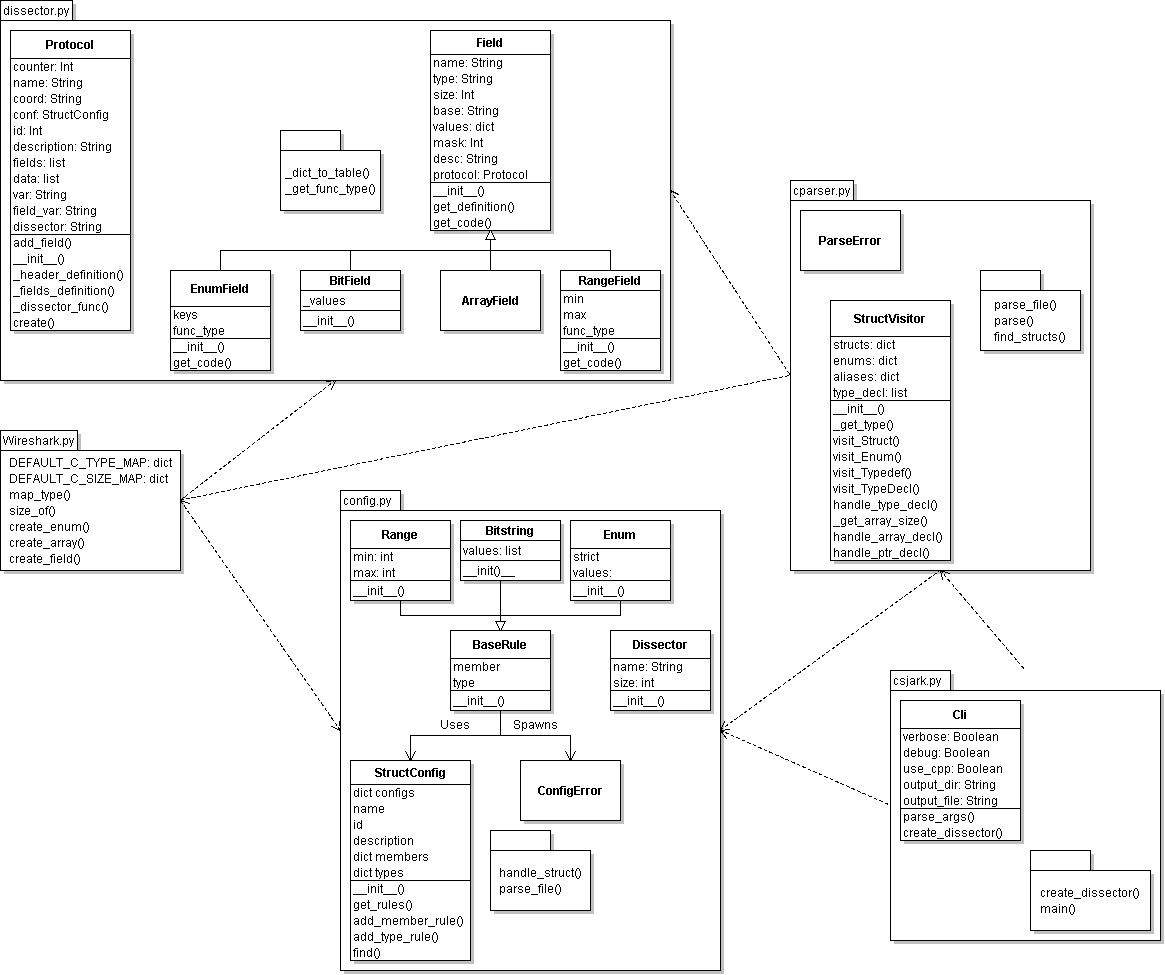
\includegraphics[width=\textwidth]{./sprints/img/class_diagram_s2}
	\caption{Class Diagram\label{fig:sp2_class}}
\end{figure}




%-----------------------
\section{Implementation}
%-----------------------


%-----------------------
\section{Sprint Testing}
%-----------------------


%--------------------------
\section{Customer Feedback}
%--------------------------


%--------------------------
\section{Sprint Evaluation}
%--------------------------


